\section{Plan-to-Do: Thrust 2 (T2). Quality Evaluation Framework for CRL Models}
\label{thrust:eval}

We aim to develop an evaluation framework for the quality of the
vectors produced by a CRL model. The evaluation is on two types: 1)
for the vectors of the {\em individual elements}, 2) for the vectors
of the {\em relations} among them. The elements in an CRL could be
{\em code token, statement, method, class, a code transformation, a
  test case, code coverage, an AST sub-tree, a PDG sub-graph, API,
  etc}. The relations among elements could be {\em the data and control
dependency, containment relation, def-use relation, inheritance
relation},~etc.

\subsection{T2 Task 1. Evaluation Framework for Vectors of Individual Elements via Vector Locality}

The key goal of the evaluation framework in this part is to measure
the quality of the vector representations for aforementioned
individual elements. Our principle includes {\em i) if two elements
  are ``similar'', their vectors must be nearby in the vector space,
  and ii) the nearby vectors must represent the ``similar'' elements}.
The notion of ``similarity'' is defined based on the abstractions used
in the given CRL model $\mathcal{M}$ under evaluation. For example, if
the CRL model aims to capture the code sequence or the AST code
structures in the input, then similarity is defined as the sequence
similarity or tree-structured similarity, e.g., via sequence edit
distance or tree editing distance, respectively. To produce the
``similar'' element for a given element for the evaluation of
$\mathcal{M}$, we rely on two research bodies in {\bf mutation} and
{\bf code clones}.

For example, a CRL aims to capture the AST code structure of the
method $m$. We will produce mutated code from $m$ by a set of {\em
  mutation operators} on the AST of the method $m$. Each mutator makes
a single structural change to the AST to produce a mutant of $m$ that
is similar to $m$.  We will make sure that the change does not create
invalid source code. A single structural change in this case could be
a tree-editing operator, such as adding/deleting a node or swapping
the order of two nodes. We will also apply the mutation operators on
the names of the program entities in $m$. We use the notion
``relatedness'', ``similarity'', and ``contextual similarity'' in
idBench~\cite{idbench}, a benchmark for the identifiers in source
code. ``Relatedness'' is defined as the names that are related to each
other, ``similarity'' as the names that are similar in meaning to each
other, and ``contextual similarity'' as the names that can be
interchanged in the same context of surrounding code.

Let us take an example of the statement $s$ \code{if (a > b) val = val
  + 1; else val = val - 1;}. We have three types of mutations.
\underline{First}, we perform regular mutation
operations. Specifically, we will apply a mutation operator to produce
a ``similar'' statement, e.g., $s'$ is \code{if (a < b) val = val + 1;
  else val = val - 1;}. We use the given CRL model to run on the
original codebase and on the codebase with the replacement of 
mutated code. We then check the top-ranked list of the vectors that
are nearest to the vector $V(s)$. If the list contains $V(s')$, we
count as a hit, otherwise it is a miss. We apply several mutation
operators to produce many pairs of such $s$ and $s'$.
\underline{Second}, we also apply the renaming by using idBench,
to replace the variables' names in a statement. For example, we
produce the mutated code by renaming the variable \code{val}: \code{if
  (a > b) value = value + 1; else value = value - 1;} because
\code{val} and \code{value} are ``contextual similar'' names. \underline{Third},
we use the code that is semantically cloned from $s$ to see if the
given CRL model can produce similar vectors for $s$ and $s'$. For
example, we produce \code{if (a <= b) val = val - 1; else val = val +
  1;}. The {\bf top-ranked accuracy} is computed as the ratio between
the number of hits over the total number of cases.

We will also measure two other metrics w.r.t. {\bf contextual
  locality}. The first one is based on the principle that {\em the
  elements in the same local compound (e.g., the statements in the
  same method) have the vectors close to one another}. For this, we
measure the cosine similarity between the vector for each element
(e.g., statement) and the mean of all vectors in a local compound
(e.g., method). We take the average of those cosine similarity
values. The second one is based on the principle that {\em the same
  element in different surrounding context must have different
  vectors}. E.g., the word {\em ``bank''} in two different contexts of
financial instituion and of a river must have different
vectors. We use clone detection to search for the exact cloned
statement in different surrounding code, and measure the difference
between each pair of those corresponding vectors.

%Context?
%1.2.1 Figure 3: average cos similarity between token vector and mean
%1.2.2 Figure 2: same unit in different sentences

\begin{wrapfigure}{l}{0.5\textwidth}
%	\vspace{-12pt}
	\centering
	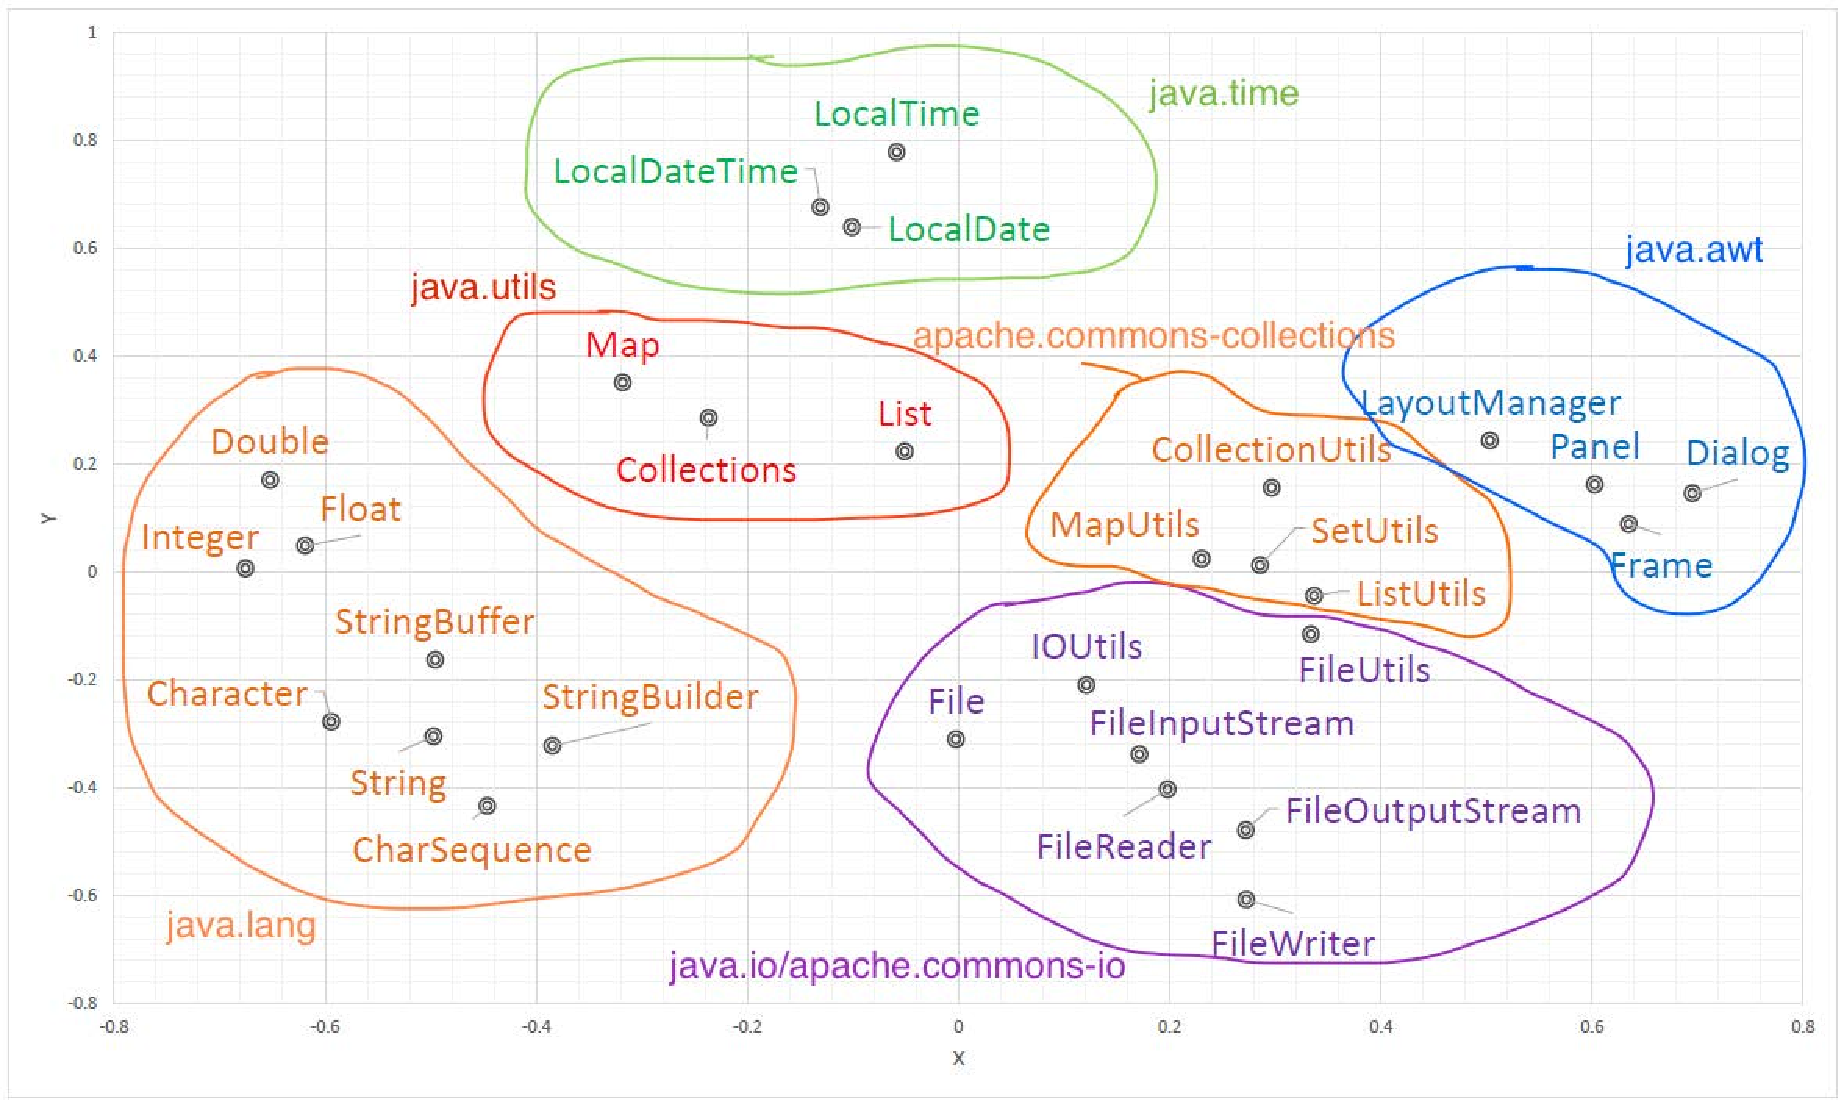
\includegraphics[width=3.2in]{graphs/PCA1}
%	\vspace{-20pt}
	\caption{2-D PCA projection of JDK and Apache API vectors}
	\label{APIspace}
%	\vspace{-10pt}
\end{wrapfigure}
In an exploratory study, we first selected some common APIs and
projected their corresponding feature vectors into a two-dimensional
space to observe the geometric arrangements among
them. Figure~\ref{APIspace} shows a PCA visualization of the vectors.
The vector space is separately divided into six clusters that
correspond to six different packages. For example, \code{String},
\code{StringBuffer} and \code{StringBuilder} in the package
\code{java.lang} have very similar embeddings since they often appear
together and are similarly described in the Java
documentation. Interestingly, API elements for file manipulation such
as \code{IOUtils} and \code{FileUtils} in Apache can be grouped in the
same cluster as \code{File} and \code{FileInputStream} in JDK. This
observation indicates that vector locality could be used in measuring
the quality of the vectors produced by an CRL model for the APIs with
similar context usages.


%the representation learned on documentations is capable of capturing
%similar contexts surrounding similar APIs to reveal the locality among
%them.
%

\subsection{T2 Task 2. Evaluation Framework for Relations among Elements via Vector Offsetting}

In NLP, vector offsetting has been shown to be able to capture some
semantic relations among words, e.g., (country, capital), (company,
product), etc. In software engineering, our preliminary work shows
that vector offsetting also holds for the vectors of the API elements.
For example, $V$(\code{Set.contains}) - $V$(\code{Set.add}) $\approx$
$V$(\code{Map.containsKey}) - $V$(\code{Map.put}), even though
different names are used.

Inspired by those results, we propose a methodology to measure the
quality of an CRL model in capturing the relations among elements as
follows. Assume that we have two statements with a data dependence:
\code{a = b + 1; c = a + 2;}.  We rely on mutation in such a way that
the data dependence is still preserved in the mutated code. For
example, we could mutate them into \code{a = b - 1; c = a - 2;}. We
will perform such mutation for many statements to produce many pairs
of original statements $s$ and mutated ones $s'$, in which their
relations have been preserved after mutation.  We then use the CRL
model under evaluation to run on the original dataset and the one with
mutated code. We will get two pairs of vectors: [$V(s_1)$ and
  $V(s'_1)$] and [$V(s_2)$ and $V(s'_2)$]. We compute the vector $V$ =
$V(s_1)$ - $V(s'_1)$ + $V(s'_2)$.  We then form the top-ranked list of
closest vectors to $V$ and check if it contains the vector
$V(s_2)$. If yes, it is a hit, otherwise it is a miss. {\bf
  Top-ranked accuracy} is measured as the ratio between the number of
hits over the total number of cases.

If an CRL model has a combination of multiple data structures for
their target, we will separately perform different mutation types to
measure how well the produced vectors capture different types of data
structures. For example, an CRL model combines the three different
types of vectors for code sequences, AST structures, and PDG graphs.
We will have different types of mutations with regard to each types of
data structures. For evaluating the relations among different elements
across different types, we will design new types of mutation operators
supporting such cross-type relations.

%\pagebreak
